% vim: set ts=4 sw=4 tw=80 noexpandtab:
%******************************************************************************%
%                                                                              %
%                   MapYourOwn.tex                                             %
%                   Made by: Kai                                               %
%                                                                              %
%******************************************************************************%

\documentclass{42-en}

%******************************************************************************%
%                                                                              %
%                                   Prologue                                   %
%                                                                              %
%******************************************************************************%

\begin{document}

\title{Map Your Own Adventure}
\subtitle{Blaze a trail}

\member {Kai}{kai@42.us.org}

\summary
{
We are very happy if you are coming to 42 campus to work on any project outside
of the ones that are written up here.
}

\maketitle

\tableofcontents

%Initialisation des headers d'exercices

\startexercices

%******************************************************************************%
%                                                                              %
%                                Ambitions                                     %
%                                                                              %
%******************************************************************************%

\chapter{Ambitions}

\begin{center}
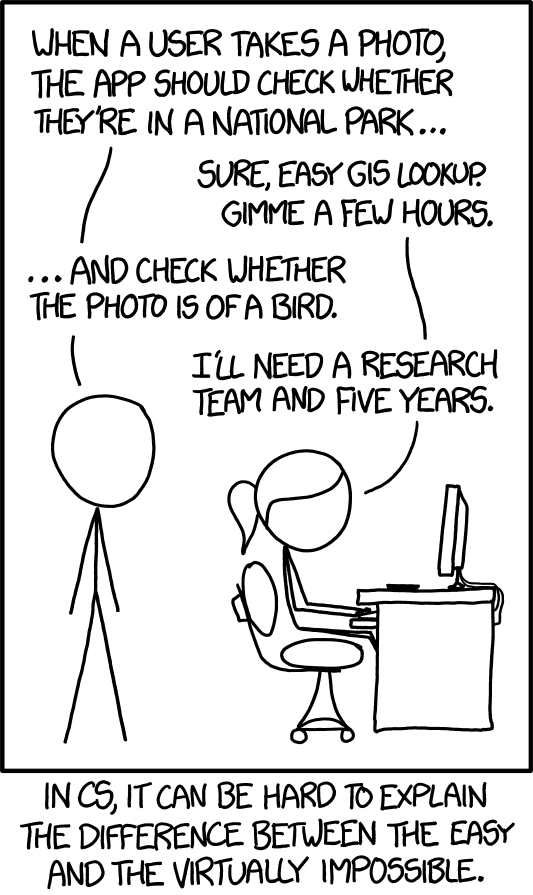
\includegraphics[width=0.6\textwidth]{xkcd_tasks.png}
\end{center}

%******************************************************************************%
%                                                                              %
%                              What to Do Here                                 %
%                                                                              %
%******************************************************************************%

\chapter{What To Do}

For this project, all you need to do is the following:

\begin{enumerate}

	\item Brainstorm something you would like to work on. If you are following a step-by-step tutorial, try planning something out that you can do to make your project special beyond the end of the tutorial.
	\item Work with your mentor to install the packages and programs you need to get your project started. Make sure that you don't run into any unsolvable obstacles in setting up your programming environment.
	\item Submit the questionnaire on the next page, filled out as a text file, and sign up for corrections with your peers. You will help inspire other students this way by showing them your ideas.

\end{enumerate}


%******************************************************************************%
%                                                                              %
%                                Questionnaire                                 %
%                                                                              %
%******************************************************************************%

\chapter{Questionnaire}

\begin{itemize}

	\item Write a paragraph - What is your project plan? What tutorials or guides are you using to get started?
	\item As a list: list some features that you are confident you can implement. (Essential part)
	\item As a list: list some features that you might be able to implement, if you have more time to work on it. (Bonus parts)
	\item As a list: What software packages, programs or platforms are required to build your project? What languages will you be using?
	\item Are you able to install these on the 42 computers? Will you be using a laptop? (Ask a mentor if you feel stuck; we may be able to let you use the Hackathon computers which have root access.)

\end{itemize}


%******************************************************************************%
%                                                                              %
%                                Corrections                                   %
%                                                                              %
%******************************************************************************%

\chapter{Corrections}

Push your text file to Vogsphere and sign up for corrections with your classmates; remember to open correction slots if you don't have any points. Go ahead and begin working on your project while you wait for corrections to complete. 

\end{document}